\section{\ac{SAT}-солверы}

Сравнивать SMT с SAT, это как сравнивать высокоуровневый ЯП с языком ассемблера.
Последний может быть куда более эффективным, но на нем труднее программировать.

SAT это аббревиатура от ``Boolean satisfiability problem''.
Проблема в том, чтобы найти такой набор переменных, которые, если их подставить в булево выражение, в результате
дадут ``истинно''.

В русскоязычной литературе используется термин ``Задача выполнимости булевых формул'' и вместо ``SAT'' иногда используют ``ВЫП''.

\subsection{CNF форма}

\ac{CNF}\footnote{\url{https://en.wikipedia.org/wiki/Conjunctive_normal_form}} это так называемая \textit{нормальная форма}.

% TODO recheck
% TODO write abt it!
%\textit{normal form} is somewhat similar to polynomials in algebra. 
%What is polynomial?
%It is a standard way to express unsystematic equations like $2x \cdot x$ as $3x$ polynomial, 
%and so you will be able to apply some operations to polynomials like summing, etc.

Любое булево выражение может быть сконвертировано в \textit{нормальную форму}, и \ac{CNF} это одна из них.
\ac{CNF}-выражение это пачка клозов (подвыражений) состоящих их литералов (или термов, переменных), операций ИЛИ и НЕ,
все из которых склеены друг с другом в полное выражение операцией И.
Вот способ запомнить: \ac{CNF} это ``И всех ИЛИ'' (или ``произведение всех сумм'')
и \ac{DNF} это ``ИЛИ всех И'' (или ``сумма всех произведений'').

Пример: $(\neg A \vee B) \wedge (C \vee \neg D)$.

$\vee$ означает ИЛИ (логическая дизьюнкция\footnote{\url{https://en.wikipedia.org/wiki/Logical_disjunction}}), 
знак ``+'' также иногда используется для ИЛИ.

$\wedge$ означает ИЛИ (логическая коньюнкция\footnote{\url{https://en.wikipedia.org/wiki/Logical_conjunction}}).
Легко запомнить: $\wedge$ выглядит как буква ``A''.
Знак ``$\cdot$'' также иногда используется для И.

$\neg$ это отрицание (НЕ).

% TODO A/B is the first clause, C/D is second

\subsection{Пример: двухбитный сумматор}
\label{adder}

В сущности, \ac{SAT}-солвер это солвер огромных булевых уравнений в CNF-форме.
Он просто выдает ответ, есть ли набор входных значений, удовлетворяющий CNF-выражению, и какие это значения должны быть.

Вот для примера двухбитный сумматор:

\begin{figure}[ht!]
\centering
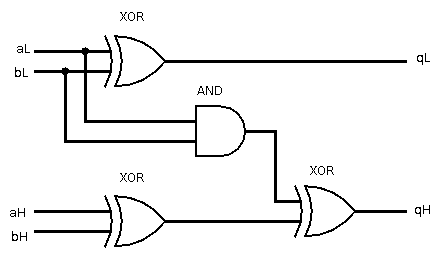
\includegraphics[scale=0.75]{SAT/adder_logisim.png}
\caption{Схема двухбитного сумматора}
\end{figure}

Сумматор здесь в самом простом возможном виде: у него нет входных и выходных переносов, и тут только 3 XOR-гейта
и один AND-гейт.
Попробуем разобраться, какой набор входных переменных заставит сумматор выставить оба выходных бита?
Просто подсчитав в уме, мы можем увидеть, что таких способа 4: $0+3=3$, $1+2=3$, $2+1=3$, $3+0=3$.
Вот также таблица истинности, с подсвеченными соответствующими рядами:

\newcommand{\HLcell}{\cellcolor{blue!25}}

\begin{center}
\begin{doublespace}
\noindent\(\begin{array}{l|llllll}
  & \text{aH} & \text{aL} & \text{bH} & \text{bL} & \text{qH} & \text{qL} \\
\hline
 \text{3+3 = 6 $\equiv $ 2 (mod 4)} & 1 & 1 & 1 & 1 & 1 & 0 \\
 \text{3+2 = 5 $\equiv $ 1 (mod 4)} & 1 & 1 & 1 & 0 & 0 & 1 \\
 \text{3+1 = 4 $\equiv $ 0 (mod 4)} & 1 & 1 & 0 & 1 & 0 & 0 \\
 \text{\HLcell{}3+0 = 3 $\equiv $ 3 (mod 4)} & \HLcell{}1 & \HLcell{}1 & \HLcell{}0 & \HLcell{}0 & \HLcell{}1 & \HLcell{}1 \\
 \text{2+3 = 5 $\equiv $ 1 (mod 4)} & 1 & 0 & 1 & 1 & 0 & 1 \\
 \text{2+2 = 4 $\equiv $ 0 (mod 4)} & 1 & 0 & 1 & 0 & 0 & 0 \\
 \text{\HLcell{}2+1 = 3 $\equiv $ 3 (mod 4)} & \HLcell{}1 & \HLcell{}0 & \HLcell{}0 & \HLcell{}1 & \HLcell{}1 & \HLcell{}1 \\
 \text{2+0 = 2 $\equiv $ 2 (mod 4)} & 1 & 0 & 0 & 0 & 1 & 0 \\
 \text{1+3 = 4 $\equiv $ 0 (mod 4)} & 0 & 1 & 1 & 1 & 0 & 0 \\
 \text{\HLcell{}1+2 = 3 $\equiv $ 3 (mod 4)} & \HLcell{}0 & \HLcell{}1 & \HLcell{}1 & \HLcell{}0 & \HLcell{}1 & \HLcell{}1 \\
 \text{1+1 = 2 $\equiv $ 2 (mod 4)} & 0 & 1 & 0 & 1 & 1 & 0 \\
 \text{1+0 = 1 $\equiv $ 1 (mod 4)} & 0 & 1 & 0 & 0 & 0 & 1 \\
 \text{\HLcell{}0+3 = 3 $\equiv $ 3 (mod 4)} & \HLcell{}0 & \HLcell{}0 & \HLcell{}1 & \HLcell{}1 & \HLcell{}1 & \HLcell{}1 \\
 \text{0+2 = 2 $\equiv $ 2 (mod 4)} & 0 & 0 & 1 & 0 & 1 & 0 \\
 \text{0+1 = 1 $\equiv $ 1 (mod 4)} & 0 & 0 & 0 & 1 & 0 & 1 \\
 \text{0+0 = 0 $\equiv $ 0 (mod 4)} & 0 & 0 & 0 & 0 & 0 & 0 \\
\end{array}\)
\end{doublespace}
\end{center}


Посмотрим, что об этом скажет SAT-солвер?

В начале, нам нужно представить наш двухбитный сумматор как CNF-выражение.

Используя Wolfram Mathematica, можно выразить 1-битное выражение для обоих выходов сумматоров:\\
\\
\textbf{\texttt{In[]:=AdderQ0[aL$\_$,bL$\_$]=Xor[aL,bL]}} \\
\textbf{\texttt{Out[]:=aL $\veebar$ bL}} \\
\\
\textbf{\texttt{In[]:=AdderQ1[aL$\_$,aH$\_$,bL$\_$,bH$\_$]=Xor[And[aL,bL],Xor[aH,bH]]}} \\
\textbf{\texttt{Out[]:=aH $\veebar$ bH $\veebar$ (aL \&\& bL)}} \\
\\
Нам нужно такое выражение, где обе части выдадут единицы.
Используя Wolfram Mathematica, найдем все возможные входы такого выражения (я склеил обе части при помощи And): \\
\\
\textbf{\texttt{In[]:=Boole[SatisfiabilityInstances[And[AdderQ0[aL,bL],AdderQ1[aL,aH,bL,bH]],\{aL,aH,bL,bH\},4]]}} \\
\textbf{\texttt{Out[]:=\{1,1,0,0\},\{1,0,0,1\},\{0,1,1,0\},\{0,0,1,1\}}} \\
\\
Да, действительно, Mathematica говорит, что здесь 4 входа, которые приведут к нужному нам результату.
Так что, Mathematica тоже может использоваться как \ac{SAT}-солвер.

Тем не менее, перейдем к CNF-форме. Используя Mathematica, сконвертируем наше выражение в CNF-форму:\\
\\
\textbf{\texttt{In[]:=cnf=BooleanConvert[And[AdderQ0[aL,bL],AdderQ1[aL,aH,bL,bH]],``CNF'']}} \\
\textbf{\texttt{Out[]:=(!aH $\|$ !bH) \&\& (aH $\|$ bH) \&\& (!aL $\|$ !bL) \&\& (aL $\|$ bL)}} \\
\\
Выглядит посложнее. Причина такой многословности в том, что \ac{CNF}-форма не поддерживает операцию исключающего
ИЛИ.
% FIXME: TeX form of the expression!

\subsubsection{MiniSat}

Для начала, попробуем MiniSat\footnote{\url{http://minisat.se/MiniSat.html}}.
Стандартный способ закодировать \ac{CNF}-выражение для MiniSat это перечислить все части ИЛИ в каждой строке.
Также, MiniSat не поддерживает имена переменных, только числа.
Перечислим наши переменные: 1 будет aH, 2 -- aL, 3 -- bH, 4 -- bL.

Вот что получилось, когда я сконвертировал выражение из Mathematica во входной файл для MiniSat:

\lstinputlisting{SAT/adder.cnf}

Две четверки в первой строке это, соответственно, число переменных и число клозов.
Так что тут 4 строки, каждая для каждого клоза ИЛИ.
Минус перед номером переменной означает что переменная инвертирована.
Отсутствие минуса -- не инвертирована.
Ноль в конце это просто оконечивающий ноль, означающий конец клоза.

Другими словами, каждая строка это ИЛИ-клоз с возможными инвертированиями,
и задача MiniSat в том, чтобы найти такой набор входных переменных, который удовлетворит все строки во входном файле.

Этот файл я назвал \textit{adder.cnf} и теперь попробуем MiniSat:

\begin{lstlisting}
% minisat -verb=0 adder.cnf results.txt
SATISFIABLE
\end{lstlisting}

Результаты в файле \textit{results.txt}:

\begin{lstlisting}
SAT
-1 -2 3 4 0
\end{lstlisting}

Это означает, что если первые две переменных (aH и aL) будут \textit{false},
и две последние переменные (bH и bL) будут \textit{true},
все \ac{CNF}-выражение будет истинно (satisfiable).
Похоже на правду: если bH и bL выставить в \textit{true}, оба бита результата также будут \textit{true}.

Как получить другие решения (instances)?
\ac{SAT}-солверы, как и \ac{SMT}-солверы, выдают только одно решение (или \textit{instance}).

MiniSat использует \ac{PRNG}, и его изначальное состояние (seed) можно задать явно.
Я попробовал разные значения, но результат всё тот же.
Тем не менее, CryptoMiniSat в этом случае может показать все возможные 4 решения, хотя и в хаотичном порядке.
Так что это не очень надежный способ.

Видимо, единственный способ, это инвертировать клоз решения и добавить его во входное выражение.
Мы получили \TT{-1 -2 3 4}, 
теперь мы можем инвертировать все значения в нем (просто поменяйте минусы: \TT{1 2 -3 -4}),
и добавим это в конец входного файла:

\begin{lstlisting}
p cnf 4 5
-1 -3 0
1 3 0
-2 -4 0
2 4 0
1 2 -3 -4
\end{lstlisting}

Получаем другой результат:

\begin{lstlisting}
SAT
1 2 -3 -4 0
\end{lstlisting}

Это означает что обе aH и aL должны быть \textit{true} и bH и bL должны быть \textit{false}, чтобы удовлетворить
входное выражение.
Снова инвертируем это решение и снова добавим:

\begin{lstlisting}
p cnf 4 6
-1 -3 0
1 3 0
-2 -4 0
2 4 0
1 2 -3 -4
-1 -2 3 4 0
\end{lstlisting}

Результат:

\begin{lstlisting}
SAT
-1 2 3 -4 0
\end{lstlisting}

aH=false, aL=true, bH=true, bL=false. Это также корректно, в соответствии с таблицей истинности.

Добавим снова:

\begin{lstlisting}
p cnf 4 7
-1 -3 0
1 3 0
-2 -4 0
2 4 0
1 2 -3 -4
-1 -2 3 4 0
1 -2 -3 4 0
\end{lstlisting}

\begin{lstlisting}
SAT
1 -2 -3 4 0
\end{lstlisting}

\textit{aH=true, aL=false, bH=false, bL=true.} Это тоже верно.

Это четвертый результат. Больше быть не должно. Что если добавим и это?

\begin{lstlisting}
p cnf 4 8
-1 -3 0
1 3 0
-2 -4 0
2 4 0
1 2 -3 -4
-1 -2 3 4 0
1 -2 -3 4 0
-1 2 3 -4 0
\end{lstlisting}

Теперь MiniSat просто говорит ``UNSATISFIABLE'' без всякой дополнительной информации в файле результатов.

Нам пример крохотный, но MiniSat может работать с огромными \ac{CNF}-выражениями.

\subsubsection{CryptoMiniSat}

Операция исключающего ИЛИ (XOR) отсутствует в CNF-форме, но она очень важна в криптографических алгоритмах.
Простейший способ представить одну единственную XOR-операцию в CNF-форме, это:
$(\neg x \vee \neg y) \wedge (x \vee y)$ -- не очень короткое выражение,
хотя, множество XOR-операций в одном выражении могут оптимизироваться лучше.

Одна значительная разница между MiniSat и CryptoMiniSat в том, что последний поддерживает
клозы с операцией XOR вместо ИЛИ,
потому что CryptoMiniSat предназначен больше для анализа криптоалгоритмов\footnote{\url{http://www.msoos.org/xor-clauses/}}.
XOR-клозы поддерживаются в CryptoMiniSat специальным образом, без трансляции в клозы ИЛИ.

Вам нужно просто прибавить ``x'' к клозу в \ac{CNF}-файле и CryptoMiniSat затем считает обычный ИЛИ-клоз как XOR-клоз.
Что до двухбитного сумматора, вот самое короткое из возможных XOR-CNF выражений, которое можно использовать
для поиска всех входных значений, где оба выходных бита выставлены:

$(aH \oplus bH) \wedge (aL \oplus bL)$

Это \TT{.cnf}-файл CryptoMiniSat:

\begin{lstlisting}
p cnf 4 2
x1 3 0
x2 4 0
\end{lstlisting}

Запускаю CryptoMiniSat с разными значениями для инициализации его \ac{PRNG} \dots

\begin{lstlisting}
% cryptominisat4 --verb 0 --random 0 XOR_adder.cnf
s SATISFIABLE
v 1 2 -3 -4 0
% cryptominisat4 --verb 0 --random 1 XOR_adder.cnf
s SATISFIABLE
v -1 -2 3 4 0
% cryptominisat4 --verb 0 --random 2 XOR_adder.cnf
s SATISFIABLE
v 1 -2 -3 4 0
% cryptominisat4 --verb 0 --random 3 XOR_adder.cnf
s SATISFIABLE
v 1 2 -3 -4 0
% cryptominisat4 --verb 0 --random 4 XOR_adder.cnf
s SATISFIABLE
v -1 2 3 -4 0
% cryptominisat4 --verb 0 --random 5 XOR_adder.cnf
s SATISFIABLE
v -1 2 3 -4 0
% cryptominisat4 --verb 0 --random 6 XOR_adder.cnf
s SATISFIABLE
v -1 -2 3 4 0
% cryptominisat4 --verb 0 --random 7 XOR_adder.cnf
s SATISFIABLE
v 1 -2 -3 4 0
% cryptominisat4 --verb 0 --random 8 XOR_adder.cnf
s SATISFIABLE
v 1 2 -3 -4 0
% cryptominisat4 --verb 0 --random 9 XOR_adder.cnf
s SATISFIABLE
v 1 2 -3 -4 0
\end{lstlisting}

Тем не менее, все 4 возможных решения, это:

\begin{lstlisting}
v -1 -2 3 4 0
v -1 2 3 -4 0
v 1 -2 -3 4 0
v 1 2 -3 -4 0
\end{lstlisting}

\dots то же, что и выдал MiniSat.

\subsection{Picosat}

По крайней мере Picosat может перечислить все возможные решения без тех костылей, которые я только что показывал:

\begin{lstlisting}
% picosat --all adder.cnf
s SATISFIABLE
v -1 -2 3 4 0
s SATISFIABLE
v -1 2 3 -4 0
s SATISFIABLE
v 1 2 -3 -4 0
s SATISFIABLE
v 1 -2 -3 4 0
s SOLUTIONS 4
\end{lstlisting}

% subsections:
\subsection{Задача о восьми ферзях}
\label{EightQueens}

Восемь ферзей это популярная задача, и она часто используется для измерения скорости работы SAT-солверов.
Нужно расставить на шахматной доске 8 ферзей так, чтобы они не атаковали друг друга.
Например:

\begin{lstlisting}
| | | |*| | | | |
| | | | | | |*| |
| | | | |*| | | |
| |*| | | | | | |
| | | | | |*| | |
|*| | | | | | | |
| | |*| | | | | |
| | | | | | | |*|
\end{lstlisting}

Попробуем разобраться, как её решить.

\subsubsection{make\_one\_hot}
\label{POPCNTOne}

Одна важная ф-ция, которую мы будем (часто) использовать это \TT{make\_one\_hot}.
Это ф-ция, которая возвращает \textit{Истинно}, если один из входов истинен, остальные ложны.
Она вернет \textit{Ложно} в остальных случаях.

В моих других примерах, я использовал Wolfram Mathematica для генерирования CNF-клозов для этого, например: \ref{minesweeper_SAT}.
Какое выражение сгенерирует Mathematica для ф-ции \TT{make\_one\_hot} для 8-и входов?

\begin{lstlisting}
(!a||!b)&&(!a||!c)&&(!a||!d)&&(!a||!e)&&(!a||!f)&&(!a||!g)&&(!a||!h)&&(a||b||c||d||e||f||g||h)&&
(!b||!c)&&(!b||!d)&&(!b||!e)&&(!b||!f)&&(!b||!g)&&(!b||!h)&&(!c||!d)&&(!c||!e)&&(!c||!f)&&(!c||!g)&&
(!c||!h)&&(!d||!e)&&(!d||!f)&&(!d||!g)&&(!d||!h)&&(!e||!f)&&(!e||!g)&&(!e||!h)&&(!f||!g)&&(!f||!h)&&(!g||!h)
\end{lstlisting}

Мы можем ясно увидеть что выражение состоит из всех возможных пар переменных (инвертированных) плюс
перечисление всех переменных (не инвертированных).
На обычном русском языке это означает: ``ни одна пара не должна быть равна двум \textit{Истинно} \textit{И}
по крайней мере одно \textit{Истинно} должно
присутствовать среди переменных''.

Вот как это работает: если две переменных будут \textit{Истино}, инвертированными они обе будут \textit{Ложно},
и этот клоз не будет
вычислен как \textit{Истинно}, а это наша конечная цель.
Если одна из переменных будет \textit{Истинно}, инвертированными, одна будет \textit{Истинно},
вторая \textit{Ложно} (хорошо).
Если обе переменных будут \textit{Ложно}, инвертированными, они обе будут \textit{Истинно} (тоже хорошо).

Вот как мы можем сгенерировать клозы для этой ф-ции используя модуль \textit{itertools} из Питона,
который также содержит много важных ф-ций из комбинаторики:

\begin{lstlisting}
    # naive/pairwise encoding   
    def AtMost1(self, lst):
        for pair in itertools.combinations(lst, r=2):
            self.add_clause([self.neg(pair[0]), self.neg(pair[1])])
       
    # make one-hot (AKA unitary) variable
    def make_one_hot(self, lst):
        self.AtMost1(lst)
        self.OR_always(lst)
\end{lstlisting}

Ф-ция \TT{AtMost1()} перечисляет все возможные пары используя ф-цию \textit{combinations()} из
\textit{itertools}.

Ф-ция \TT{make\_one\_hot()} делает то же самое, только добавляет последний клоз, который заставляет иметь хотя бы одну
переменную, равную Истинно.

Какие клозы будут сгенерированы для 5-и переменных (1..5)?

\lstinputlisting{SAT/8queens/popcnt1.cnf}

Да, это все возможные пары чисел 1..5 + все 5 чисел.

Можем посмотреть все решения используя Picosat:

\begin{lstlisting}
% picosat --all popcnt1.cnf

s SATISFIABLE
v -1 -2 -3 -4 5 0
s SATISFIABLE
v -1 -2 -3 4 -5 0
s SATISFIABLE
v -1 -2 3 -4 -5 0
s SATISFIABLE
v -1 2 -3 -4 -5 0
s SATISFIABLE
v 1 -2 -3 -4 -5 0
s SOLUTIONS 5
\end{lstlisting}

Действительно, 5 возможных решений.

\subsubsection{Восемь ферзей}

Теперь вернемся назад к восьми ферзям.

Мы можем назначить 64 переменных для $8 \cdot 8=64$ клеток.
Клетка на которой есть ферзь будет равна \textit{Истинно}, пустая клетка будет \textit{Ложно}.

Проблема расположения неатакующих (друг друга) ферзей на шахматной доске (любого размера), на обычном русском
языке может быть выражена так:

\begin{itemize}
\item один единственный ферзь должен присутствовать в каждом ряду;

\item один единственный ферзь должен присутствовать в каждом столбце;

\item или один ферзь должен присутствовать на каждой диагонали, или вовсе отсутствовать (пустые диагонали могут быть
и в правильном решении).
\end{itemize}

Эти правила можно перевести так:

\begin{itemize}
\item make\_one\_hot(каждый ряд)==\textit{Истинно}

\item make\_one\_hot(каждый столбец)==\textit{Истинно}

\item AtMost1(каждая диагональ)==\textit{Истинно}
\end{itemize}

Теперь мы должны перечислить ряды, столбцы и диагонали, и собрать все клозы:

\lstinputlisting{SAT/8queens/8queens.py}
( \url{https://github.com/DennisYurichev/SAT_SMT_article/blob/master/SAT/8queens/8queens.py} )

Возможно, ф-ция \TT{gen\_diagonal()} выглядит не очень эстетично:
она перечисляет также поддиагонали более длинных диагоналей, которые уже были раннее.
Чтобы не было повторяющихся клозов, глобальная переменная \textit{clauses} это не список, а множество,
которое может содержать в себе только уникальные данные.

Также, я использовал ф-цию \TT{AtMost1} для каждого столбца, это поможет генерировать чуть меньше клозов.
Каждый столбец будет содержать ферзя в любом случае, это следует из первого правила (\TT{make\_one\_hot} для каждого ряда).

После запуска, получаем CNF-файл с 64-я переменными и 736-я клозами (\url{https://github.com/DennisYurichev/SAT_SMT_article/blob/master/SAT/8queens/8queens.cnf}).
Вот одно из решений:

\begin{lstlisting}
% python 8queens.py
len(clauses)= 736
| | | |*| | | | |
| | | | | | |*| |
| | | | |*| | | |
| |*| | | | | | |
| | | | | |*| | |
|*| | | | | | | |
| | |*| | | | | |
| | | | | | | |*|
\end{lstlisting}

Как много здесь возможных решений?
Picosat говорит что 92, что действительно корректное число решений (\url{https://oeis.org/A000170}).

Скорость Picosat не очень впечатляет, вероятно потому что ему приходится выводить все решения.
Моему древнему нетбуку с Intel Atom 1.66GHz, понадобилось 34 для перечисления всех решений для шахматной доски
$11 \cdot 11$ 
(2680 решения),
что намного медленнее, чем моя прямолинейная программа полного перебора: \url{https://yurichev.com/blog/8queens/}.
Тем не менее, для поиска первого решения, Picosat работает крайне быстро (как и другие SAT-солверы).

Эта SAT-задача также достаточно проста, чтобы её можно было легко решить при помощи моего простейшего
SAT-солвера, работающего на базе поиска с возвратом (\textit{backtracking}):
\ref{SAT_backtrack}.

\subsubsection{Подсчет всех решений}

Мы получаем решение, инвертируем его и добавляем как новый констрайнт.
На обычном русском языке это звучит ``найди решение, котороые также не ровно тому, что мы только что нашли/добавили''.
Мы добавляем их последовательно, и процесс замедляется --- потому что размер проблемы (\textit{instance}) растет 
и SAT-солверу всё труднее находить новое решение.

\subsubsection{Пропуск симметрических решений}

Мы также можем добавлять повернутое и отраженное (горизонтально) решение, чтобы пропускать симметрические решения.
Делая так, мы получаем 12 решений для доски 8*8, 46 для 9*9, итд.
Это \url{https://oeis.org/A002562}.


\subsection{Простейший SAT-солвер в \textasciitilde{}120 строках}
\label{SAT_backtrack}

Это простейший SAT-солвер работающий на базе поиска с возвратом (\textit{backtracking}) (не \ac{DPLL}), написанный
на Питоне.
Он использует тот же поиск с возвратом, который можно найти в простейших солверах Судоку и задачи о восьми ферзях.
Он работает значительно медленнее, но, из-за предельной простоты, он также может подсчитывать количество решений.
Например, он может подсчитать все решения для задачи о восьми ферзях (\ref{EightQueens}).

Также, имеется 70 решений для ф-ции POPCNT4
\footnote{\url{https://github.com/DennisYurichev/SAT_SMT_article/blob/master/SAT/backtrack/POPCNT4.cnf}}
(ф-ция истинна, если любые из её 4-х входов из 8-и истинны):

\begin{lstlisting}
SAT
-1 -2 -3 -4 5 6 7 8 0
SAT
-1 -2 -3 4 -5 6 7 8 0
SAT
-1 -2 -3 4 5 -6 7 8 0
SAT
-1 -2 -3 4 5 6 -7 8 0
...

SAT
1 2 3 -4 -5 6 -7 -8 0
SAT
1 2 3 -4 5 -6 -7 -8 0
SAT
1 2 3 4 -5 -6 -7 -8 0
UNSAT
solutions= 70
\end{lstlisting}

Солвер также тестировался на моем взломщике Сапёра основанном на SAT (\ref{minesweeper_SAT}),
и заканчивает работу в разумное время (хотя и медленнее чем MiniSat раз в \textasciitilde{}10).

На б\'{о}льших \ac{CNF}-задачах он зависает.

Исходный код:
% TODO: translate to RU:
\lstinputlisting{SAT/backtrack/SAT_backtrack.py}

Как вы видите, всё что он делает, это перечисляет все возможные решения, но отсекает поисковое дерево настолько рано,
насколько это возможно.
Это и есть поиск с возвратом (\textit{backtracking}).

Файлы: \url{https://github.com/DennisYurichev/SAT_SMT_article/tree/master/SAT/backtrack}.

Некоторые комментарии: \url{https://www.reddit.com/r/compsci/comments/6jn3th/simplest_sat_solver_in_120_lines/}.


%\input{SAT/list_RU}

